This section documents the results of the Turbine in Wake test case. This test case was run twice, once without Feed Forward Derating Control enabled and once with Feed forward Derating Control. The following figures and text analyze the behavior of the upwind turbine (which was identical in both runs of the Offset Turbine test case), the behavior of the downwind turbine when Feed Forward Derating Control is not enabled, and the behavior of the downwind turbine when Feed Forward Derating Control is enabled.

Figure \ref{fig6-27} shows wind speed in the computational domain at several key moments when Feed Forward Derating Control is not enabled. Each image in Figure \ref{fig6-14} was generated by taking a horizontal cross section through the center of the computational domain then trimming the cross section to remove regions that were far from the turbines in the downwind or horizontal directions. White lines have been superimposed on the images to show the locations and approximate sizes of the turbine rotors. At t=300 s we see that the upwind turbine is operating in a steady, uniform 12 m/s wind. The downwind turbine is subject to a lower and less consistent wind speed because it is in the wake of the upwind turbine. At t = 400 s the Extreme Coherent Gust enters the computational domain. We see at t = 420 s that the gust has begun to propagate through the domain from left to right. At t = 480 s we see that the gust has recently reached the upwind turbine. At t = 540 s we see the gust arriving at the downwind turbine. In the t = 540 s image we can also see that there is no wake trailing the upwind turbine. This indicates that the upwind turbine has shut down. At t = 660 s we see that the gust has continued to propagate downstream and there is no wake trailing the downwind turbine, which indicates that it has also shut down. A similar set of images was generated for the Turbine in Wake test case with Feed Forward Derating Control (but is not shown here). Those images look very similar, except at t = 600 s. In the t = 600 s image a wake is visible trailing the downwind turbine, which indicates that Feed Forward Derating Control prevents the downwind turbine from shutting down.

 \begin{figure}[!htbp] 
	\centering
		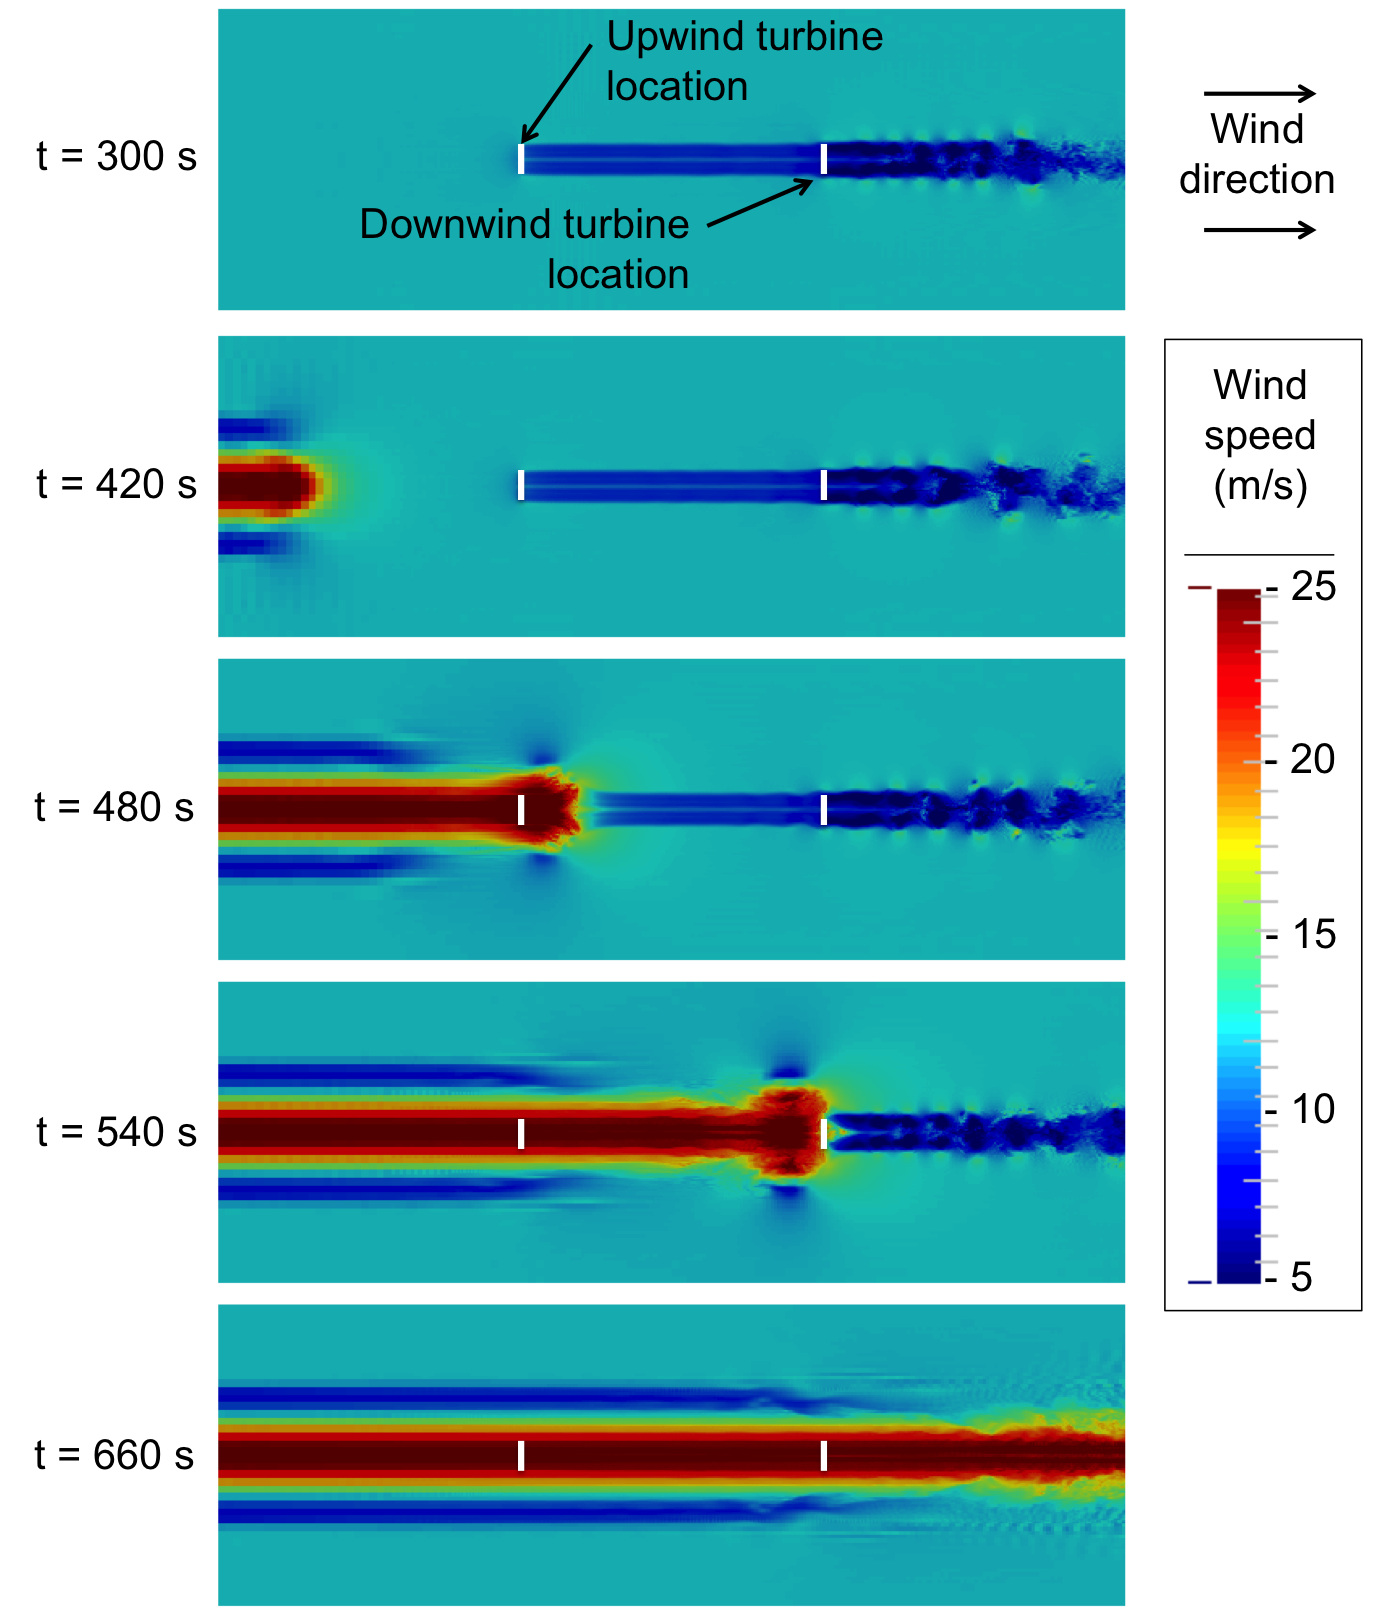
\includegraphics[width = \linewidth]{Figures/ch6Figures/fig6-27.png}

	\caption{Wind speeds at several moments for the Turbine in Wake test case without feed forward control.}
	\label{fig6-27} 
\end{figure}

 Figures \ref{fig6-28} through \ref{fig6-32} show the rotor speed, power generation, blade pitch, blade root bending moment, and tower base fore-aft bending moment of the turbines. In Figure \ref{fig6-28} we see that the upwind turbine is initially rotating at a constant rate of 12.1 RPM. This is expected for a turbine in 12 m/s wind because it is operating in region 3 control. The downwind turbine, which is in the wake of the upwind turbine,  has a lower rotational speed with some fluctuations. The lower rotational speed indicates that the downwind turbine is operating in region 2 control, which does not track a constant rotational speed. Region 2 control uses generator torque to vary rotational speed in an attempt to maximize power generation. The Extreme Coherent gust reaches the upwind turbine at approximately t = 450 s, triggering an emergency overspeed shutdown at t = 466.7 s. If Feed Forward Derating Control is enabled, a signal is sent to the downwind turbine instructing it to derate by 11.12\% beginning at t = 478.7 s and return to full rated operation at t = 624.2 s. Between t = 478.7 s and t = 508.7 s the downwind turbine with Feed Forward Derate Control smoothly reduces it's rotor speed and power generation, while the downwind turbine without feed forward control continues to operate according to normal region 2 control. The Extreme Coherent Gust reaches the downwind turbine at approximately t = 520 s. The downwind turbine without feed forward control exceeds the 15\% overspeed limit at t = 538.6 s and an emergency overspeed shutdown is initiated. The downwind turbine with Feed Forward Derate Control experiences a maximum overspeed of 11.12\% , which does not cause an emergency overspeed shutdown. Between t = 624.2 s and t = 654.2 s the downwind turbine transitions back to full rated operation.


 Figures \ref{fig6-28} through \ref{fig6-32} show the rotor speed, power generation, blade pitch, blade root bending moment, and tower base fore-aft bending moment of the turbines. We see in figures \ref{fig6-28} and \ref{fig6-29} that the upwind turbine is initially rotating at a constant rate of 12.1 RPM and producing 5,000 kW of power. This is expected for a turbine in 12 m/s wind because it is operating in region 3 control. The downwind turbine, which is in the wake of the upwind turbine,  has a lower rotational speed and a lower power generation. The downwind turbine also has some fluctuations in rotor speed and power generation. The lower rotational speed indicates that the downwind turbine is operating in region 2 control, which does not track a constant rotational speed. Region 2 control uses generator torque to vary rotational speed in an attempt to maximize power generation. The Extreme Coherent gust reaches the upwind turbine at approximately t = 450 s, triggering an emergency overspeed shutdown at t = 466.7 s. If Feed Forward Derating Control is enabled, a signal is sent to the downwind turbine instructing it to derate by 11.12\% beginning at t = 478.7 s and return to full rated operation at t = 624.2 s. Between t = 478.7 s and t = 508.7 s the downwind turbine with Feed Forward Derate Control smoothly reduces it's rotor speed and power generation, while the downwind turbine without feed forward control continues to operate according to normal region 2 control. The Extreme Coherent Gust reaches the downwind turbine at approximately t = 520 s. The downwind turbine without feed forward control experiences a large spike in rotor speed and power generation (a much larger change than what the upwind turbine experiences) as it is briefly put into region 3 operation. At t = 538.6 s the downwind turbine without feed forward control exceeds the 15\% overspeed limit and an emergency overspeed shutdown is initiated. The downwind turbine with Feed Forward Derate Control experiences a maximum overspeed of 11.12\% , which does not cause an emergency overspeed shutdown. Between t = 624.2 s and t = 654.2 s the downwind turbine transitions back to full rated operation.

\begin{figure}[!htbp] 
	\centering
		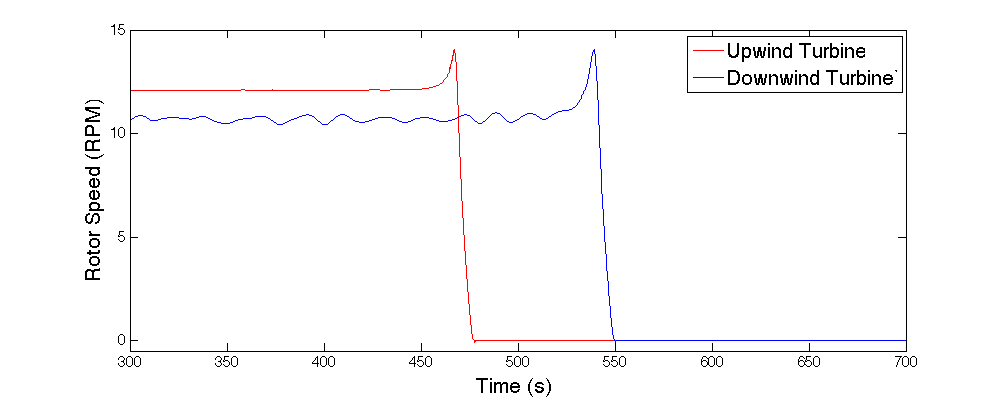
\includegraphics[width = \linewidth]{Figures/ch6Figures/fig6-28.png}
	\caption{Rotor speed during the Turbine in Wake test case without feed forward control.}
	\label{fig6-28}
\end{figure}

\begin{figure}[!htbp] 
	\centering
		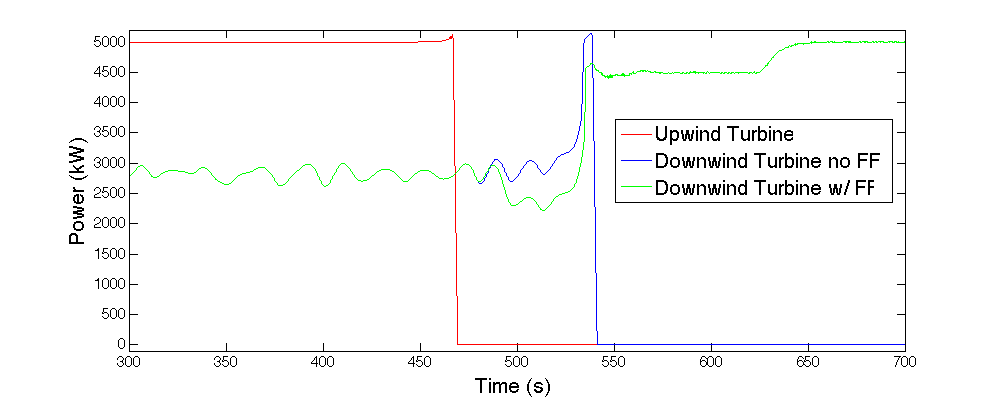
\includegraphics[width = \linewidth]{Figures/ch6Figures/fig6-29.png}

	\caption{Power generation during the Turbine in Wake test case without feed forward control.}
	\label{fig6-29}
\end{figure}

On average the downwind turbine is producing approximately 2800 kW of power prior to the Extreme Coherent Gust. This is 44\% less power than the upwind turbine, which illustrates that wake effects can have a very large impact on power production.The downwind power generation seen in Figure \ref{fig6-27} is consistent with the rotor speeds seen in Figure \ref{fig6-28}, is consistent with results in Chapter \ref{Chapter4}, and is consistent with results that other researchers have published for wake effects 20R downstream of a turbine in turbulence free conditions. For an NREL 5MW turbine, power production of 2800 kW corresponds to an effective incoming wind speed of 9.4 m/s. This indicates that the upwind turbine wake is causing an average wind velocity deficit of 22\%  at the downwind turbine (20R downstream).This is similar to the velocity deficit shown in Figure \ref{fig5-5}-b. A 22\% wind velocity deficit is also consistent with the findings of Troldborg et al. for RANS (Reynolds Averaged Navier Stokes) simulations of an NREL 5MW turbine \cite{troldborg2015}, and LES (Large Eddy Simulation) based simulations of a 2MW NEG Micon NM80 turbine \cite{troldborg2010,troldborg2010b}. Furthermore, a 22\% wind velocity deficit is consistent with the dynamic wake meandering model described by Madsen et al. \cite{madsen2010}. These publications looked at a variety of turbine operating conditions and several noteworthy trends were found. Velocity deficit decreases as downstream distance increases. Velocity deficits decrease faster in turbulent conditions than in turbulence free conditions. Velocity deficits are largest when the turbine is in region 2 operation. When in region 3 operation, velocity deficit decreases as wind speed increases.


Figure \ref{fig6-30} shows the blade pitch of the turbines. Initially, the upwind turbine has a blade pitch of 4.8\degree and the downwind turbine has a pitch of 0\degree. As the upwind turbine begins to experience increased wind speed (at t = ~450 s) it's blade pitch increases in an effort to maintain a constant rotational speed of 12.1 RPM. The upwind turbine's blade pitch is at 15.3\degree when the emergency shutdown procedure is initiated at t = 466.7 s. After the emergency shutdown is initiated blade pitch increases to 90\degree at a rate of 8\degree /s. The downwind turbine begins to experience increased wind speed at t = ~520 s. The downwind turbine without feed forward control maintains a blade pitch of 0\degree until the rotor speed increases to 12.1 RPM. Once the rotor speed reaches 12.1 RPM the turbine transitions from region 2 control to region 3 control and increases blade pitch in an effort to maintain that rotational speed. The upwind turbine's blade pitch is at 10.4\degree when the emergency shutdown procedure is initiated at t = 538.6 s. The downwind turbine with Feed Forward Derating Control increases blade pitch from 0\degree to 2.6\degree when the turbine is derated (starting at t = 478.7 s). The gust causes an increase and some oscillation in blade pitch, with the blade pitch eventually settling to approximately 25.5\degree. When the turbine is returned to full rated operation, starting at t = 624.2 s, blade pitch decreases to 23.1\degree.

As the downwind turbine without feed forward control begins to experience increased wind speed (at t = ~520 s) the turbine 

\begin{figure}[!htbp] 
	\centering
		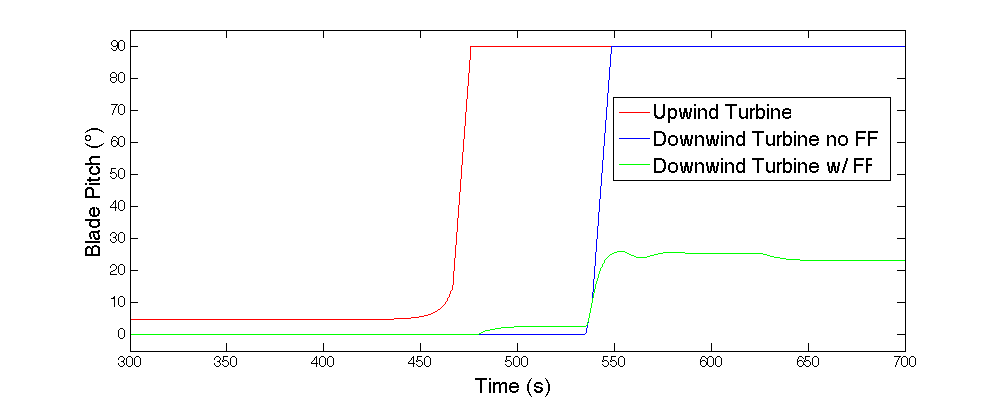
\includegraphics[width = \linewidth]{Figures/ch6Figures/fig6-30.png}

	\caption{Blade pitch during the Turbine in Wake test case without feed forward control.}
	\label{fig6-30}
\end{figure}

Figures \ref{fig6-31} shows blade root bending moment (BRM). The BRM loading behavior for the upwind turbine looks very similar to what we saw in the Offset Turbine test cases (Figure \ref{fig6-18}). Before the Extreme Coherent Gust arrives, BRM loading cycles are very consistent in both shape and magnitude. When the upwind turbine begin to experience higher wind speeds and blade pitch begins to increase, the BRM loading cycle maintains it's shape but begins to decrease in magnitude. Durring the emergency shutdown process the shape of the BRM loading cycle changes and larger fluctuations in BRM can be seen. When the rotor comes to a halt the BRM settles to a constant value. Early in the simulation, because of wake effects, BRM loading cycles for the downwind turbine are less consistent in shape and BRM has a slightly lower magnitude on average. For the downwind turbine without feed forward control the gust causes an increase in BRM (at t = ~520 s). This brief period of high loading is because the turbine maintains a 0\degree blade pitch angle until the rotor speed increases to 12.1 RPM. The combination of high wind speed and low blade pitch angle causes very high aerodynamic loading on the turbine blade. When emergency shutdown is initiated the shape of the BRM loading cycle then becomes irregular and there are a few large fluctuations before BRM settles to a constant value. Note that the downwind turbine without feed forward control experiences larger BRM loads than the upwind turbine durring the emergency overspeed shutdown. The downwind turbine with Feed Forward Derating Control experiences a small decrease in BRM loads when the turbine is derated at t = 478.7 s. There is a brief increase in BRM loads when the Extreme Coherent Gust reaches the turbine at approximately t = 520 s. This period of high loading occurs while the downwind turbine is transitioning from region 2 derated control to region 3 derated control. By t = 550 s the mean BRM decreases to approximately 3 MNm (~60\% below the initial mean BRM) and the cyclical fluctuations in BRM have increased to approximately 4 MNm (~140\% above the initial magnitude of fluctuations).

\begin{figure}[!htbp] 
	\centering
		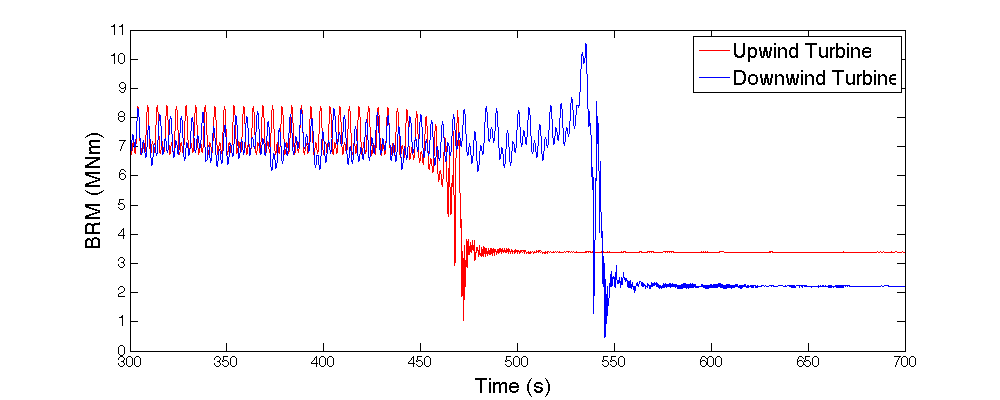
\includegraphics[width = \linewidth]{Figures/ch6Figures/fig6-31.png}

	\caption{Blade root bending moment (BRM) during the Turbine in Wake test case without feed forward control.}
	\label{fig6-31}
\end{figure}

In Figure \ref{fig6-32} we see that the tower base fore-aft bending moments for the upwind turbine is initially constant at approximately 48 MNm. The tower base bending moment is highly dependent on the aerodynamic loading, which is highly dependent on blade pitch. As wind speeds begin to increase and blade pitches begin to increase we see a smooth reduction in tower fore-aft bending moment. The emergency shutdown process causes a short period of cyclical loading, including one large loading cycle where the tower base fore-aft bending moment goes from 47 MNm to -41 MNm. Early in the simulation the downwind turbine has slightly lower tower base fore-aft bending moments, but has more fluctuations in loading. This is due to wake effects. The downwind turbine without feed forward control experiences a sharp increase in loading when the gust arrives at t = ~520 s. As discussed in the previous paragraph, this is because the downwind turbine maintains a 0\degree blade pitch angle until the rotor speed increases to 12.1 RPM. The combination of high wind speed and low blade pitch angle causes very high aerodynamic loading. The emergency shutdown process causes a short period of cyclical loading, including an abrupt change from 76 MNm to -46 MNm. The downwind turbine with Feed Forward Derating Control is derated at t = 478.7 s. This causes a reduction in tower base fore-aft bending moment. This is consistent with a reduction in aerodynamic loading on the turbine rotor due to increasing blade pitch. When the gust arrives loading sharply increases to 63.4 MNm. This brief period of high loading occurs as the turbine transitions from region 2 to region 3 control. By t = 550 s the mean tower fore-aft bending moment has decreased to approximately 2 MNm. However, a cyclic loading component persists through the end of the simulation. If we zoom in on these high frequency oscillations, we see that the loading has a very similar shape to the cyclic BRM loading seen in Figure \ref{fig6-31}, but has a frequency three times higher. Since the turbine rotor has three blades, this indicates that the higher magnitude BRM oscillations seen near the end of the simulation are causing the high frequency oscillations in tower loading. 


\begin{figure}[!htbp] 
	\centering
		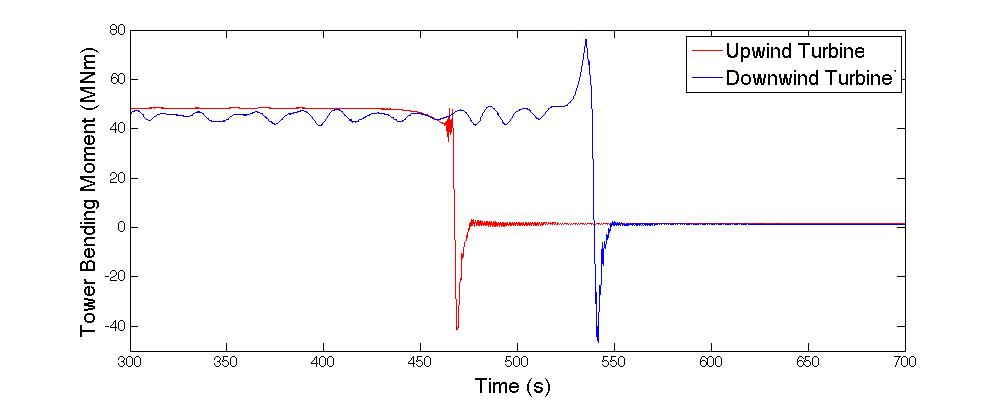
\includegraphics[width = \linewidth]{Figures/ch6Figures/fig6-32.png}

	\caption{Tower base fore-aft bending moment during the Turbine in Wake test case without feed forward control.}
	\label{fig6-32}
\end{figure}


Table \ref{Table6-6} summarizes several important performance metrics for the turbines. The downwind turbine without feed forward control has much higher Damage Equivalent Loads (DEL) than the upwind turbine. If we look at figures \ref{fig6-31} and \ref{fig6-32} it is easy to see where the discrepancy in DEL is coming from. The downwind turbine has much higher loads and more loading fluctuations due to the Extreme Coherent Gust and and the subsequent emergency shutdown. However, I think it's useful to discuss what this means for the turbines and what the root cause of this discrepancy is. This discrepancy means that an Extreme Coherent Gust large enough to cause emergency shutdown is more damaging to a turbine in a wake than to a turbine that is not in a wake. The downwind turbine has to endure the change in wind speed caused by the gust in addition to a change in wind speed due to the upwind turbine shutting down. The upwind turbine is initially operating in 12 m/s wind then experiences a suden increase of 13 m/s to a 25 m/s wind speed. The downwind turbine is initially operating in an average wind speed of 9.4 m/s then experiences a suden increase of 15.6 m/s to a 25 m/s wind speed. The upwind turbine and the downwind turbine without feed forward control experience similar maximum overspeeds. Finally, we see that the upwind turbine produces 38.88 KWh more energy than the downwind turbine without feed forward control. The downwind turbine without feed forward control operates for a longer period of time before it experiences an emergency overspeed shutdown. However, as we see in Figure \ref{fig6-29}, it generates less power than the upwind turbine due to wake effects.

Feed Forward Derating Control improves turbine behaviour in all four performance metrics. Tower base fore-aft bending moment DEL has been reduced by 58.1 MNm, which is a reduction of 56\%. This is likely because the downwind turbine with feed forward derating control does not experience the very large magnitude loading cycles observed immediately prior to and durring emergency shutdown. Blade root bending moment DEL has been reduced by 15\% despite the turbine operating for a longer period of time and enduring a larger quantity of BRM loading cycles. Maximum overspeed has been reduced to 11.7\%, which will not induce an emergency shutdown. Energy generation has been increased by 201.14 KWh.

It is important to note that the difference in energy generation could be much larger in real world operation. These simulations end at t = 700 s, but beyond that time the downwind turbine with feed forward derating control would continue to generate 5 MW (or ~1.4 KWH per second). The downwind turbine without feed forward derating control would not generate any power until it was returned to service. That turbine may be shut down for much longer than the 158.8 seconds captured in these simulations.


\begin{table}[!htbp]
\centering
\begin{tabular}{c|cccccccccc}
\hline
\hline
                                                                &  & \begin{tabular}[c]{@{}c@{}}Tower base\\ DEL(MNm)\end{tabular} & & \begin{tabular}[c]{@{}c@{}}Blade root\\ DEL(MNm)\end{tabular} &  & \begin{tabular}[c]{@{}c@{}}Max\\ Overspeed(\%)\end{tabular} &  &  \begin{tabular}[c]{@{}c@{}}Energy\\ Gen.(kWh)\end{tabular}\\ 
\hline
\begin{tabular}[c]{@{}c@{}}Upwind \\ Turbine \end{tabular}      &  & 76.8                                                          & & 6.92                                                          &  & 16.12                                 				      &  &  233.39                                                     \\
\\
\begin{tabular}[c]{@{}c@{}}Downwind \\ Turbine \end{tabular}    &  & 104.0                                                         & & 9.49                                                          &  & 16.03                                                       &  &  194.51                                                     \\
\\
\hline
\hline                             
\end{tabular}
\caption{Turbine performance metrics for the Turbine in Wake test case without feed forward control.}
 \label{Table6-6}
\end{table}
